\subsection{Lines and Planes}

\FromC{\From Section 1.5 of \VCT.}

\BEN
\item 
Find vector equations for the following lines.
\begin{enumerate}
\item Find the vector equation for the line that passes through the points (-1,2,1), and (3,-2,1).
\item Find the vector equation for the line that has parametric equations $x=2+2t, y=9t, z=5+t$.
\end{enumerate}
% -  -  -  -  -  -  -  -  -  -  -  -  -  -  -  -  -  -  -  -  -  -  -  -  -  -  -  -  -  -  
\item 
Calculate the following angles.
\begin{enumerate}
\item Calculate the angle between the vectors $\BM -1\\ 0 \\ 1 \EM$, and $\BM 0 \\ -2 \\ 2 \EM$.
\item Calculate the angle between the vector $\mathbf{x}=\BM 1 \\ 0 \\ 2 \EM$ and the plane $2x+y-z=0$.
\end{enumerate}
% -  -  -  -  -  -  -  -  -  -  -  -  -  -  -  -  -  -  -  -  -  -  -  -  -  -  -  -  -  -  
\item 
\Emph{Distance Between a Point and a Line}\\
Find the distance between the point (1,0,0) and the line $x=1, y=t, z=1$.
% -  -  -  -  -  -  -  -  -  -  -  -  -  -  -  -  -  -  -  -  -  -  -  -  -  -  -  -  -  -  
\item 
\Emph{Distance Between a Point and a Plane}\\
Consider the point $(-1,C,1)$ and the plane $2x+y-z=3$, where $C$ is an unknown constant. Find all possible values of $C$ such that the distance between the given point and plane is equal to $\sqrt{6}$. 
% -  -  -  -  -  -  -  -  -  -  -  -  -  -  -  -  -  -  -  -  -  -  -  -  -  -  -  -  -  -  
\item 
Consider the points $P, Q, R$ \\
\begin{align*}
P &=(1,0,3)\\
Q &=(2,2,3)\\
R &=(0,0,-1)
\end{align*}
\begin{enumerate}
\item Find a vector that is perpendicular to the plane that passes through these points.
\item Find the area of the triangle $\bigtriangleup PQR$.
\item Find a point $S$ so that a unique plane that passes through $P, Q$, and $S$ cannot be found. Describe why you cannot find a unique plane that passes through $P, Q$, and $S$. 
\end{enumerate}
%% -  -  -  -  -  -  -  -  -  -  -  -  -  -  -  -  -  -  -  -  -  -  -  -  -  -  -  -  -  -  
%\item % QUESTION 
%Find two unit vectors perpendicular to vectors $\begin{bmatrix} 1 \\ 0\\4 \end{bmatrix}$ and $\mathbf{i}-2\mathbf{j}+\mathbf{k}$. 
%% -  -  -  -  -  -  -  -  -  -  -  -  -  -  -  -  -  -  -  -  -  -  -  -  -  -  -  -  -  -  
%\item 
%Suppose vectors $\mathbf{a}$, $\mathbf{b}$, and $\mathbf{c}$ are in $\mathbb{R}^3$, and \textbf{a}$\ne 0$. If \textbf{a}$\cdot\mathbf{b}=\mathbf{a}\cdot\mathbf{c}$, does it follow that $\mathbf{b}=\mathbf{c}$? Briefly explain your answer. 
% -  -  -  -  -  -  -  -  -  -  -  -  -  -  -  -  -  -  -  -  -  -  -  -  -  -  -  -  -  -  
\item % EQUATIONS OF PLANES 
\Emph{Equations of Planes}\\
Find the equation of the plane that
\begin{enumerate}
\item passes through the points (-1,2,1), (3,-2,1), and (-1,1,-1).
\item passes through the point (-1,2,1) and contains the line $x=y=z$.
\end{enumerate}
% -  -  -  -  -  -  -  -  -  -  -  -  -  -  -  -  -  -  -  -  -  -  -  -  -  -  -  -  -  -  
\item % QUESTION 
Suppose we have two planes $2x+y-z=3$ and $x+3y+z=0$. Find the line of intersection between these two planes, and find the equation of the plane that passes through the line of intersection and through the point $(0,0,0)$.
% -  -  -  -  -  -  -  -  -  -  -  -  -  -  -  -  -  -  -  -  -  -  -  -  -  -  -  -  -  -  
\item % QUESTION
Suppose that $L_1$ is a line in $\R^3$.
\begin{enumerate}
\item Is it possible to find another line, $L_2$, that is parallel $L_1$, and intersects $L_1$ at only one point? Show that it is  possible, or show that it is not possible with a counterexample.
\item Suppose that there is a line $L_3$ that is is parallel to $L_1$, and that a plane $P$ includes both $L_1$ and $L_3$. Is it always true that there exists a plane that is perpendicular to $P$? 
\end{enumerate}
% -  -  -  -  -  -  -  -  -  -  -  -  -  -  -  -  -  -  -  -  -  -  -  -  -  -  -  -  -  -  
%\item % QUESTION 
%Consider the following vectors in $\R^2$:
%\begin{align*}
%\mathbf{a} = \begin{bmatrix} 1/\sqrt{2} \\ -1/\sqrt{2} \end{bmatrix}, \quad
%\mathbf{b} = \begin{bmatrix} 1/\sqrt{2} \\ 1/\sqrt{2} \end{bmatrix}, \quad
%\mathbf{r} =  \begin{bmatrix} 3 \\ 1 \end{bmatrix}.
%\end{align*}
%\begin{enumerate}
%\item Verify that $\mathbf{a}$ and $\mathbf{b}$ are perpendicular unit vectors. 
%\item Use your results from part (a) to find constants $C_1$ and $C_2$ so that $\mathbf{r}=C_1\mathbf{a}+C_2\mathbf{b}$.
%\end{enumerate}
%% -  -  -  -  -  -  -  -  -  -  -  -  -  -  -  -  -  -  -  -  -  -  -  -  -  -  -  -  -  -  
%\item % QUESTION 
%Suppose that $\mathbf{a}$, $\mathbf{b}$ and $\mathbf{c}$ are nonzero vectors in $\R^3$. Prove the following statements.
%\begin{enumerate}
%\item If $||\mathbf{a} + \mathbf{b}||^2 = ||\mathbf{a}||^2 + ||\mathbf{b}||^2$, then vectors $\mathbf{a}$ and $\mathbf{b}$ are perpendicular. 
%\item If $\mathbf{a}\times\mathbf{b} = \mathbf{a}\times\mathbf{c}$ and $\mathbf{a}\cdot\mathbf{b} = \mathbf{a}\cdot\mathbf{c}$, then $\mathbf{b} =\mathbf{c}$.
%\end{enumerate}
%% -  -  -  -  -  -  -  -  -  -  -  -  -  -  -  -  -  -  -  -  -  -  -  -  -  -  -  -  -  -  
%\item 
%Suppose that $\mathbf{a}$, $\mathbf{b}$ and $\mathbf{c}$ are nonzero vectors in $\R^3$. Identify which of the following statements are meaningless and which statements are not meaningless. Explain your reasoning.
%\begin{enumerate}
%\item  $\mathbf{a}\cdot (\mathbf{b} \times \mathbf{c})$ 
%\item  $\mathbf{a}\cdot (\mathbf{b} \cdot \mathbf{c})$ 
%\item  $\mathbf{a}\times (\mathbf{b} \cdot \mathbf{c})$ 
%\item  $\mathbf{a}\times (\mathbf{b} \times \mathbf{c})$ 
%\end{enumerate}
%% -  -  -  -  -  -  -  -  -  -  -  -  -  -  -  -  -  -  -  -  -  -  -  -  -  -  -  -  -  -  
%\item \textbf{Application to Mechanics, Part I} \\
%Torque plays a fundamental role in many branches of engineering. It is vector that describes rotation rotation about a point or axis due to an applied force. If you haven't yet encountered torque, its mathematical definition is straightforward:
%\begin{quote}
%The torque, $\boldsymbol\tau$, about a pivot point $P$, that is produced by a force \textbf{F} applied at a point $Q$, is defined as $\boldsymbol\tau = \mathbf{r} \times \mathbf{F}$, where $\mathbf{r}=\overrightarrow{PQ}$.
%\end{quote}
%Torque is a vector that is produced by an applied force. For example, suppose that a force $\MB{F}=\frac{1}{2}\MB{i} + 0\MB{j} + 0\MB{k}$ is applied at the point $(1,C,0)$, about the pivot point (1,0,0), where $C\in\R$ is a constant. The resulting torque is simply 
%\begin{align*}
%\boldsymbol\tau =   
%\begin{vmatrix}
%   \MB{i} &  \MB{j} &  \MB{k} \\
%   1-1 &  C-0 &  0 \\
%   0.5 & 0 &  0 \\
%  \end{vmatrix}=-\frac{C}{2}\MB{k}
%\end{align*} 
%A plot of the applied force and produced torque vectors is shown below.
%\begin{figure}[!htbp]
%  \begin{center}
%    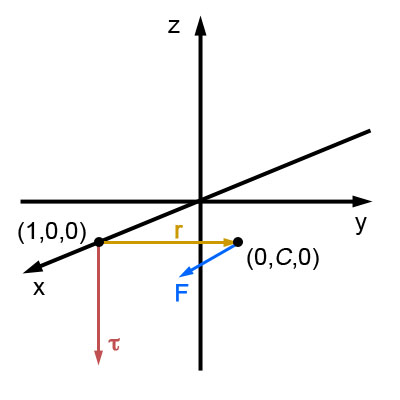
\includegraphics[width=0.5\textwidth]{ImgTorqueExample.jpg}
%  \end{center}
%\end{figure}
%
%Note that the magnitude of the torque vector is $||\boldsymbol\tau|| = C/2$, and that if we increase the value of $C$, two things happen: the applied force moves further away from the pivot point, and the magnitude of the produced torque increases. \\\\
%% Consider that:
%%\begin{itemize}
%%\item intuitively, it is easier to rotate a screwdriver with a \textbf{large} handle than it is to rotate a screwdriver a small handle. If the 
%%\item It is easier to spin a large wheel by pushing on its edge, rather than pushing on some point in the middle of the wheel. Moreover, we 
%%\end{itemize}
%\textbf{Units}\\
%When \textbf{F} has units of Newtons (N), and $\MB{r}$ has units of meters (m), torque has units of $\text{N}\cdot\text{m}$.\\\\
%\textbf{Questions}\\
%Suppose that a bicycle has pedal arms that are 0.14 m long, and that a constant downward force of $100 \text{ N}$ is applied by a cyclist on one pedal.  Let $\theta \in [0,360^{\circ})$ be the angle between the vertical and the pedal arm, as shown in the figure below. 
%\begin{figure}[!htbp]
%  \begin{center}
%    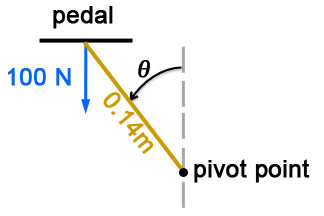
\includegraphics[width=0.4\textwidth]{ImgBicycle.jpg}
%      \caption{\small{The pedal arm (orange) rotates about the pivot point. The angle it makes with the vertical direction is $\theta$, measured counter-clockwise. A constant downward force of 100 N is applied to the pedal, which is attached to the other end of the pedal arm.}}
%  \end{center}
%\end{figure}
%\BEN
%  \item Determine the magnitude of the torque about the pivot point when $\theta$ is $30^{\circ}$ and when $\theta$ is $90^{\circ}$. Your answers should include the units of measurement. 
%  \item Determine the magnitude of the torque about the pivot point for any $\theta$. Your answer should be a function of $\theta$.  
%  \item What value(s) of $\theta$ minimize the produced torque? Briefly explain why. You should not need to compute any derivatives to answer this question. 
%\EEN
%Naturally, the torque vector can also be a function of time. In our bicycle example, the torque that is produced by the cyclist could change continuously as the pedal rotates about the pivot point. We will revisit the concept of torque as a vector function in a later assignment, after we have defined vector functions and their derivatives. 
%
%% -  -  -  -  -  -  -  -  -  -  -  -  -  -  -  -  -  -  -  -  -  -  -  -  -  -  -  -  -  -  

\EEN